\documentclass[a4paper]{article}
%\usepackage[affil-it]{authblk}
\usepackage[backend=bibtex,style=numeric]{biblatex}
\usepackage{graphicx}
\usepackage{amsmath}
\usepackage{geometry}
\usepackage{caption}
\usepackage{amssymb}
\usepackage{float}
\usepackage{ctex}
\geometry{margin=1.5cm, vmargin={0pt,1cm}}
\setlength{\topmargin}{-1cm}
\setlength{\paperheight}{29.7cm}
\setlength{\textheight}{25.3cm}

\begin{document}
% ==================================================
\title{Numerical Analysis Homework 3}

\author{罗开诚 Luo Kaicheng 3220103383
  \thanks{Electronic address: \texttt{3220103383@zju.edu.com}}}
%\affil{(Information and Computational Science 2201), Zhejiang University}

\date{Due time: \today}

\maketitle

\begin{abstract}
    Solutions to various numerical analysis problems.
\end{abstract}

% ============================================

\section*{I}
$s'(x)=-3(2-x)^2 x\in [1,2]$\\
$s''(x)=6(2-x) x\in [1,2]$\\
Substitute to get\\
$s''(1)=6,s'(1)=-3$\\
$p\in P_3, p(0)=0,p(1)=1,p'(1)=-3 ,p''(1)=6$\\
Construct divided difference\\
x||f\\
0 0\\
1 1 1 \\
1 1 -3 -4\\
1 1 -3  3 7\\
$p(x)=0+x-4x(x-1)+7x(x-1)^2=7x^3-18x^2+12x$\\
Substitute s(x)\\
s''(2)=0\\
s''(0)=-36\\
Therefore, it is not a natural cubic spline\\

\section*{II}
(a)\\
By Theorem 3.14, the spline space is of dimension \( n+1 \), but currently there are only \( n \) equations.\\
There are many polynomials that satisfy the existing conditions.\\
One construction is given here. Let $s'(x_1)=m_1$\\
In $[x_1,x_2]$ have $s(x)=f(x_2)+(x-x_2)*\frac{f(x_1)-f(x_2)}{x_1-x_2}+(x-x_1)(x-x_2)\frac{(x_1-x_2)m_1-(f(x_1)-f(x_2))}{(x_1-x_2)^2}$\\
Get $s'(x_2)=\frac{2(f(x_1)-f(x_2))-(x_1-x_2)*m_1}{x_1-x_2}$\\
By $s(x)=f(x_{i+1})+(x-x_{i+1})*\frac{f(x_i)-f(x_{i+1})}{x_i-x_{i+1}}+(x-x_i)(x-x_{i+1})\frac{(x_i-x_{i+1})m_i-(f(x_i)-f(x_{i+1}))}{(x_i-x_{i+1})^2} x\in [x_i.x_{i+1}]$\\
Construct recursively. And for different $m_1$ there are different results.\\
(b)
Construct divided difference\\
$x||f$\\
$x_{i+1},f_{i+1}$\\
$x_i,f_i ,\frac{f_i-f_{i+1}}{x_i-x_{i+1}}$\\
$x_i,f_i, m_i,\frac{(x_i-x_{i+1})m_i-(f(x_i)-f(x_{i+1}))}{(x_i-x_{i+1})^2}$\\
Construct to get\\
$p_i(x)=f(x_{i+1})+(x-x_{i+1})*\frac{f(x_i)-f(x_{i+1})}{x_i-x_{i+1}}+(x-x_i)(x-x_{i+1})\frac{(x_i-x_{i+1})m_i-(f(x_i)-f(x_{i+1}))}{(x_i-x_{i+1})^2} x\in [x_i.x_{i+1}]$\\
(c)\\
In $[x_1,x_2]$ have $s(x)=f(x_2)+(x-x_2)*\frac{f(x_1)-f(x_2)}{x_1-x_2}+(x-x_1)(x-x_2)\frac{(x_1-x_2)m_1-(f(x_1)-f(x_2))}{(x_1-x_2)^2}$\\
Get $s'(x_2)=\frac{2(f(x_1)-f(x_2)-(x_1-x_2)*m_1)}{x_1-x_2}$\\
Known $m_i$, substitute into $[x_i,x_{i+1}]$ to get the function on the interval.\\
$s(x)=f(x_{i+1})+(x-x_{i+1})*\frac{f(x_i)-f(x_{i+1})}{x_i-x_{i+1}}+(x-x_i)(x-x_{i+1})\frac{(x_i-x_{i+1})m_i-(f(x_i)-f(x_{i+1}))}{(x_i-x_{i+1})^2} x\in [x_i.x_{i+1}]$\\
Can calculate $m_{i+1}=\frac{2(f(x_i)-f(x_{i+1}))-(x_i-x_{i+1})*m_i}{x_i-x_{i+1}}$\\
So it can be calculated recursively\\

\section*{III}
$s \in S_3^2$\\
Need to make $s''(-1)=0,s''(1)=0,s(1)=-1$\\
$s'(x)=3c(x+1)^2 ,x\in[-1,0]$\\
$s''(x)=6c(x+1)$\\
$s''(0)=6c,s'(0)=3c,s(0)=1+c,s(1)=-1$\\
Construct divided difference\\
x||f\\
1 -1\\
0 1+c -2-c\\
0 1+c 3c -2-4c\\
0 1+c 3c 3c -2-7c\\
$s_2(x)=-1+(-2-c)(x-1)+(-2-4c)x(x-1)+(-2-7c)x^2(x-1)$\\
Calculate the second derivative\\
$s_2''(1)=-12-36c=0$\\
$c=-\frac{1}{3}$\\

\section*{IV}
$f(x)=cos(\frac{\pi}{2}x)$\\
(a)\\
$f(-1)=0,f(0)=1,f(1)=0$\\
$f''(-1)=f''(1)=0$\\
By Lemma 3.4\\
$M_0+2M_1+M_2=6f[-1,0,1]=-6$\\
$M_1=-3$\\
Let $f=1+a_1x+a_2x^2+a_3x^3$ on [-1,0].\\
$f''(0)=2a_2=M_1,f(-1)=1-a_1+a_2-a_3=0,f''(-1)=2a_2-6a_3=0$\\
Solve the system of linear equations to get $f=1-\frac{3}{2}x^2-\frac{1}{2}x^3$\\
Similarly on [0,1], let $f=1+a_1x+a_2x^2+a_3x^3$\\
$f''(0)=2a_2=M_1,f(1)=1+a_1+a_2+a_3=0,\\
f''(1)=2a_2+6a_3=0$\\
$f=1-\frac{3}{2}x^2+\frac{1}{2}x^3$\\
In summary, on $x \in [-1,0]$\\
$f=1-\frac{3}{2}x^2-\frac{1}{2}x^3$\\
On $x\in [0,1]$\\
$f=1-\frac{3}{2}x^2+\frac{1}{2}x^3$\\
After verification, it meets the criteria.\\

(b)\\
On $x \in [-1,0]$\\
$s''(x)=-3-3x$\\
On $x \in [0,1]$\\
$s''(x)=-3+3x$\\
$\int_{-1}^1 [s''(x)]^2 \, dx =\int_{-1}^0 [-3-3x]^2 \, dx+\int_{0}^1 [-3+3x]^2 \, dx =6 $\\
(i)\\
By the Lagrange interpolation formula, get g(x)\\
$g(x)=0*\frac{(x-0)(x-1)}{(-1-0)(-1-1)}+1*\frac{(x-(-1))(x-1)}{(0-(-1))(0-1)}+0*\frac{(x+1)(x-0)}{(1-(-1))(1-0)}$\\
$g(x)=1-x^2,g''(x)=-2$\\
$\int_{-1}^1 [g''(x)]^2 \, dx =8>\int_{-1}^1 [s''(x)]^2 \, dx=6$ so it meets the condition\\
(ii)\\
Let $g(x)=f(x)$\\
$\int_{-1}^1 [g''(x)]^2 \, dx=\frac{\pi^4}{16}>\frac{97}{16}>\int_{-1}^1 [s''(x)]^2 \, dx=6$ so it meets the condition\\

\section*{V}


(a)\\
$B_i^{n+1}(x) = \frac{x - t_{i-1}}{t_{i+n} - t_{i-1}} B_i^n(x) + \frac{t_{i+n+1} - x}{t_{i+n+1} - t_i} B_{i+1}^n(x). $\\
The hat function at $t_i$ is\\
\[
\hat{B}_i(x) = 
\begin{cases} 
\frac{x - t_{i-1}}{t_i - t_{i-1}} & x \in (t_{i-1}, t_i], \\
\frac{t_{i+1} - x}{t_{i+1} - t_i} & x \in (t_i, t_{i+1}], \\
0 & \text{otherwise}.
\end{cases}
\]
Substitute to get\\
$B_i^{2}(x) = \frac{x - t_{i-1}}{t_{i+1} - t_{i-1}} \hat{B}_i^n(x) + \frac{t_{i+2} - x}{t_{i+2} - t_i} \hat{B}_{i+1}^n(x). $\\
For $x \in (t_{i-1},t_i]$\\
$B_i^{2}(x)=\frac{x - t_{i-1}}{t_{i+1} - t_{i-1}}\frac{x-t_{i-1}}{t_i-t_{i-1}}+\frac{t_{i+n+1} - x}{t_{i+n+1} - t_i}*0=\frac{(x-t_{i-1})^2}{(t_{i+1}-t_{i-1})(t_i-t_{i-1})}$\\
For $x \in (t_{i},t_{i+1}]$\\
$B_i^{2}(x) = \frac{x - t_{i-1}}{t_{i+1} - t_{i-1}} \frac{t_{i+1}-x}{t_{i+1}-t_i} + \frac{t_{i+2} - x}{t_{i+2} - t_i} \frac{x-t_i}{t_{i+1}-t_i}=\frac{(x - t_{i-1})(t_{i+1}-x)}{(t_{i+1} - t_{i-1})(t_{i+1}-t_i)}  + \frac{(t_{i+2} - x)(x-t_i)}{(t_{i+2} - t_i)(t_{i+1}-t_i)} .$\\
For $x \in (t_{i+1},t_{i+2}]$\\
$B_i^{2}(x) =\frac{x - t_{i-1}}{t_{i+1} - t_{i-1}}*0+\frac{t_{i+2} - x}{t_{i+2} - t_i} \frac{t_{i+2}-x}{t_{i+2}-t_{i+1}}=\frac{(t_{i+2}-x)^2}{(t_{i+2} - t_i)(t_{i+2}-t_{i+1})}.$\\
Consistent with the conclusion in the book.\\
(b)\\
On $x \in (t_{i-1},t_i]$,\\
$\frac{d}{dx}B^2_i(x)=\frac{2(x-t_{i-1})}{(t_{i+1}-t_{i-1})(t_i-t_{i-1})}$\\
The left derivative at $t_i$ is $\frac{2}{(t_{i+1}-t_{i-1})}$, and the left derivative is continuous.\\
On $x \in (t_{i},t_{i+1}]$,\\
$\frac{d}{dx}B^2_i(x)= \frac{t_{i+1}+t_{i-1}-2x}{(t_{i+1} - t_{i-1})(t_{i+1}-t_i)}  + \frac{t_{i+2}+t_i-2x}{(t_{i+2} - t_i)(t_{i+1}-t_i)} .$\\
The right derivative at $t_i$ is $lim_{\epsilon->0^{+}}\frac{B^2_i(t_i+\epsilon)-B^2_i(t_i)}{\epsilon}=lim_{\epsilon->0^{+}}\frac{\frac{(t_i+\epsilon - t_{i-1})(t_{i+1}-t_i+\epsilon)}{(t_{i+1} - t_{i-1})(t_{i+1}-t_i)}  + \frac{(t_{i+2} - t_i+\epsilon)(t_i+\epsilon-t_i)}{(t_{i+2} - t_i)(t_{i+1}-t_i)}-\frac{(t_i-t_{i-1})^2}{(t_{i+1}-t_{i-1})(t_i-t_{i-1})}}{\epsilon}=\frac{2}{(t_{i+1}-t_{i-1})}$\\
And the derivative is continuous on $(t_{i-1},t_i]$, so the left derivative equals the right derivative at $t_i$, and both sides are continuous.\\
Also, the left derivative at $t_{i+1}$ is $\frac{t_{i-1}-t_{i+1}}{(t_{i+1} - t_{i-1})(t_{i+1}-t_i)}  + \frac{t_{i+2}+t_i-2t_{i+1}}{(t_{i+2} - t_i)(t_{i+1}-t_i)}=\frac{-2}{t_{i+2}-t_i}$\\
On $x \in (t_{i+1},t_{i+2}]$,\\
$\frac{d}{dx}B^2_i(x)=\frac{2(x-t_{i+2})}{(t_{i+2}-t_{i})(t_{i+2}-t_{i+1})}$\\
The right derivative at $t_{i+1}$ is $lim_{\epsilon->0^{+}}\frac{B^2_i(t_{i+1}+\epsilon)-B^2_i(t_{i+1})}{\epsilon}=lim_{\epsilon->0^{+}}\frac{\frac{(t_{i+2}-t_{i+1}-\epsilon)^2}{(t_{i+2} - t_i)(t_{i+2}-t_{i+1})}-\frac{(t_{i+2}-t_{i+1})}{(t_{i+2} - t_i)}}{\epsilon}=\frac{-2}{(t_{i+2}-t_{i})}$\\
So at $t_{i+1}$, the left derivative equals the right derivative, and both sides are continuous, proven.\\
(c)
From the derivative values calculated in (b), the derivatives at $t_i,t_{i+1}$ are not 0.\\
On $x \in (t_{i-1},t_i)$,\\
If $\frac{d}{dx}B^2_i(x)=\frac{2(x-t_{i-1})}{(t_{i+1}-t_{i-1})(t_i-t_{i-1})}=0,x=t_{i-1}$, does not meet the condition\\
On $x \in (t_{i},t_{i+1}]$,\\
Let $\frac{d}{dx}B^2_i(x)= \frac{t_{i+1}+t_{i-1}-2x}{(t_{i+1} - t_{i-1})(t_{i+1}-t_i)}  + \frac{t_{i+2}+t_i-2x}{(t_{i+2} - t_i)(t_{i+1}-t_i)} =0.$\\
There is a unique solution $t=\frac{t_{i+1}t_{i+2}-t_{i}t_{i-1}}{t_{i+1}+t_{i+2}-t_{i}-t_{i-1}}$\\
And $t-t_i=\frac{(t_{i+1}-t_i)(t_{i+2}-t_i)}{t_{i+1}+t_{i+2}-t_{i}-t_{i-1}}>0$\\
$t_{i+1}-t=\frac{(t_{i+1}-t_i)(t_{i+1}-t_{i-1})}{t_{i+1}+t_{i+2}-t_{i}-t_{i-1}}>0$\\
So the solution is on $x \in (t_{i},t_{i+1}]$ meets the condition, the conclusion is valid.\\
(d)
When \( x = t_{i-1} \), \( B_i^2(x) = 0 \) \\
When \( x \in (t_{i-1}, t_i] \), \( \frac{d}{dx}B^2_i(x) = \frac{2(x-t_{i-1})}{(t_{i+1}-t_{i-1})(t_i-t_{i-1})} > 0 \) \\
\( B_i^2(x) \leq B_i^2(t_i) = \frac{t_i-t_{i-1}}{t_{i+1}-t_{i-1}} < 1 \) \\
And \( B_i^2(x) = \frac{(x-t_{i-1})^2}{(t_{i+1}-t_{i-1})(t_i-t_{i-1})} > 0 \) holds. \\
When \( x \in [t_i, t_{i+1}] \), \( B_i^2(x) \) is continuous on this closed interval and has an extreme point. If the maximum point \( x \) satisfies \( B^2_i(x) \geq 1 \) \\
Considering \( B_i^2(t_i) = \frac{t_i-t_{i-1}}{t_{i+1}-t_{i-1}} < 1 \), \( B_i^2(t_{i+1}) = \frac{(t_{i+2}-t_{i+1})}{(t_{i+2} - t_i)} < 1 \) \\
Thus \( x \in (t_i, t_{i+1}) \), the derivative exists, so it must be 0. There is only one point with a derivative of 0 in \( (t_i, t_{i+1}) \). \\
From (c) \( x = \frac{t_{i+1}t_{i+2}-t_{i}t_{i-1}}{t_{i+1}+t_{i+2}-t_{i}-t_{i-1}} \) \\
Corresponding \( B^2_i(x) = \frac{\frac{(t_{i+1}-t_i)(t_{i+2}-t_i)}{t_{i+1}+t_{i+2}-t_{i}-t_{i-1}}}{t_{i+1} - t_{i-1}} \frac{\frac{(t_{i+1}-t_i)(t_{i+1}-t_{i-1})}{t_{i+1}+t_{i+2}-t_{i}-t_{i-1}}}{t_{i+1}-t_i} + \frac{t_{i+2} - t}{t_{i+2} - t_i} \frac{\frac{(t_{i+1}-t_i)(t_{i+2}-t_i)}{t_{i+1}+t_{i+2}-t_{i}-t_{i-1}}}{t_{i+1}-t_i} \) \\
\( = \frac{(t_{i+2}-t_i)^2}{((t_{i+2}-t_i)+(t_{i+1}-t_{i-1}))^2} < 1 \) contradiction. Therefore, the maximum point function value is less than 1. \\
The minimum point is similar. If the minimum point \( x \) satisfies \( B^2_i(x) < 0 \) \\
Considering \( B_i^2(t_i) = \frac{t_i-t_{i-1}}{t_{i+1}-t_{i-1}} > 0 \), \( B_i^2(t_{i+1}) = \frac{(t_{i+2}-t_{i+1})}{(t_{i+2} - t_i)} > 0 \) \\
Thus \( x \in (t_i, t_{i+1}) \), the derivative exists, so it must be 0. There is only one point with a derivative of 0 in \( (t_i, t_{i+1}) \). \\
From (c) \( x = \frac{t_{i+1}t_{i+2}-t_{i}t_{i-1}}{t_{i+1}+t_{i+2}-t_{i}-t_{i-1}} \) \\
Corresponding \( B^2_i(x) = \frac{\frac{(t_{i+1}-t_i)(t_{i+2}-t_i)}{t_{i+1}+t_{i+2}-t_{i}-t_{i-1}}}{t_{i+1} - t_{i-1}} \frac{\frac{(t_{i+1}-t_i)(t_{i+1}-t_{i-1})}{t_{i+1}+t_{i+2}-t_{i}-t_{i-1}}}{t_{i+1}-t_i} + \frac{t_{i+2} - t}{t_{i+2} - t_i} \frac{\frac{(t_{i+1}-t_i)(t_{i+2}-t_i)}{t_{i+1}+t_{i+2}-t_{i}-t_{i-1}}}{t_{i+1}-t_i} \) \\
\( = \frac{(t_{i+2}-t_i)^2}{((t_{i+2}-t_i)+(t_{i+1}-t_{i-1}))^2} > 0 \) contradiction. Therefore, the minimum point function value is greater than or equal to 0. \\
When \( x \in (t_{i+1}, t_{i+2}] \) the derivative is \\
\( \frac{d}{dx}B^2_i(x) = \frac{2(x-t_{i+2})}{(t_{i+2}-t_{i})(t_{i+2}-t_{i+1})} \leq 0 \) \\
Thus \( B^2_i(x) \geq B^2_i(t_{i+2}) = 0 \) \\
And \( B^2_i(x) = \frac{(t_{i+2}-x)^2}{(t_{i+2} - t_i)(t_{i+2}-t_{i+1})} < \frac{(t_{i+2}-t_{i+1})^2}{(t_{i+2} - t_i)(t_{i+2}-t_{i+1})} < 1 \) \\
In summary, the conclusion holds. \\

(e)
\begin{figure}[H]
  \centering
  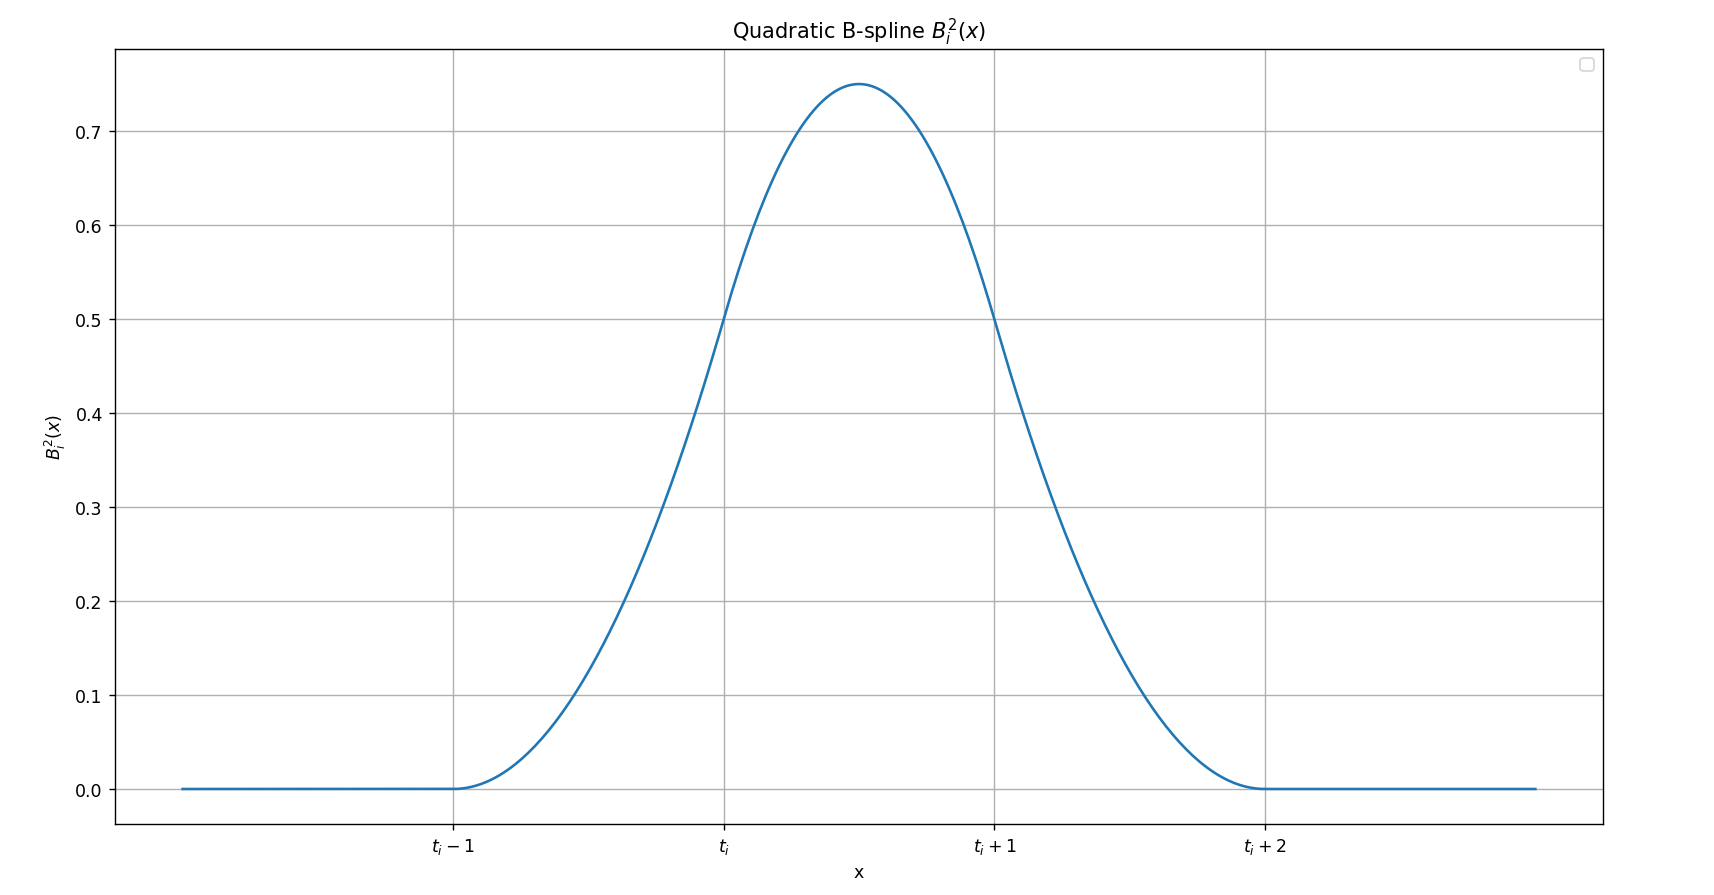
\includegraphics[width=0.8\textwidth]{plot.jpg}
\end{figure}

\section*{VI}
Prove $(t_{i+2} - t_{i-1})[t_{i-1}, t_i, t_{i+1}, t_{i+2}](t - x)_+^2 = B_i^2.$\\
Construct divided difference\\
$t_{i-1} (t_{i-1} - x)_+^2$\\
$t_{i}, (t_{i} - x)_+^2,\frac{(t_{i} - x)_+^2-(t_{i-1} - x)_+^2}{t_{i}-t_{i-1}}$\\
$t_{i+1},(t_{i+1} - x)_+^2,\frac{(t_{i+1} - x)_+^2-(t_{i} - x)_+^2}{t_{i+1}-t_{i}},\frac{\frac{(t_{i+1} - x)_+^2-(t_{i} - x)_+^2}{t_{i+1}-t_{i}}-\frac{(t_{i} - x)_+^2-(t_{i-1} - x)_+^2}{t_{i}-t_{i-1}}}{t_{i+1}-t_{i-1}}$\\
$t_{i+2},(t_{i+2} - x)_+^2,\frac{(t_{i+2} - x)_+^2-(t_{i+1} - x)_+^2}{t_{i+2}-t_{i+1}},\frac{\frac{(t_{i+2} - x)_+^2-(t_{i+1} - x)_+^2}{t_{i+2}-t_{i+1}}-\frac{(t_{i+1} - x)_+^2-(t_{i} - x)_+^2}{t_{i+1}-t_{i}}}{t_{i+2}-t_i}$\\
$[t_{i-1}, t_i, t_{i+1}, t_{i+2}](t - x)_+^2=\frac{\frac{\frac{(t_{i+2} - x)_+^2-(t_{i+1} - x)_+^2}{t_{i+2}-t_{i+1}}-\frac{(t_{i+1} - x)_+^2-(t_{i} - x)_+^2}{t_{i+1}-t_{i}}}{t_{i+2}-t_i}-\frac{\frac{(t_{i+1} - x)_+^2-(t_{i} - x)_+^2}{t_{i+1}-t_{i}}-\frac{(t_{i} - x)_+^2-(t_{i-1} - x)_+^2}{t_{i}-t_{i-1}}}{t_{i+1}-t_{i-1}}}{t_{i+2}-t_{i-1}}$\\
$(t_{i+2} - t_{i-1})[t_{i-1}, t_i, t_{i+1}, t_{i+2}](t - x)_+^2=\frac{\frac{(t_{i+2} - x)_+^2-(t_{i+1} - x)_+^2}{t_{i+2}-t_{i+1}}-\frac{(t_{i+1} - x)_+^2-(t_{i} - x)_+^2}{t_{i+1}-t_{i}}}{t_{i+2}-t_i}-\frac{\frac{(t_{i+1} - x)_+^2-(t_{i} - x)_+^2}{t_{i+1}-t_{i}}-\frac{(t_{i} - x)_+^2-(t_{i-1} - x)_+^2}{t_{i}-t_{i-1}}}{t_{i+1}-t_{i-1}}$\\
For $x \in (t_{i-1},t_i]$, $(t_{i+2} - x)_+^2=(t_{i+2} - x)^2,(t_{i+1} - x)_+^2=(t_{i+1} - x)^2\\
,(t_{i} - x)_+^2=(t_{i} - x)^2,(t_{i-1} - x)_+^2=0$ substitute into the original formula to get\\
$LHS=\frac{(t_{i+2} - x)^2-(t_{i+1} - x)^2}{(t_{i+2}-t_{i+1})(t_{i+2}-t_i)}-\frac{(t_{i+1} - x)^2-(t_{i} - x)^2}{(t_{i+1}-t_{i})(t_{i+2}-t_i)}-\frac{(t_{i+1} - x)^2-(t_{i} - x)^2}{(t_{i+1}-t_{i})(t_{i+1}-t_{i-1})}+\frac{(t_{i} - x)^2}{(t_{i}-t_{i-1})(t_{i+1}-t_{i-1})}$\\
$=1-\frac{t_{i+1}+t_{i}-2x}{t_{i+1}-t_{i-1}}+\frac{(t_{i} - x)^2}{(t_{i}-t_{i-1})(t_{i+1}-t_{i-1})}$\\
$=\frac{x^2+t_i^2-2xt_{i-1}-t_i^2+t_{i-1}^2}{(t_{i}-t_{i-1})(t_{i+1}-t_{i-1})}=\frac{(t_{i-1} - x)^2}{(t_{i}-t_{i-1})(t_{i+1}-t_{i-1})}=B_i^2$

For $x \in (t_{i},t_{i+1}]$, $(t_{i+2} - x)_+^2=(t_{i+2} - x)^2,(t_{i+1} - x)_+^2=(t_{i+1} - x)^2,(t_{i} - x)_+^2=0,(t_{i-1} - x)_+^2=0$ substitute into the original formula to get\\
$LHS=\frac{(t_{i+2} - x)^2-(t_{i+1} - x)^2}{(t_{i+2}-t_{i+1})(t_{i+2}-t_i)}-\frac{(t_{i+1} - x)^2}{(t_{i+1}-t_{i})(t_{i+2}-t_i)}-\frac{(t_{i+1} - x)^2}{(t_{i+1}-t_{i})(t_{i+1}-t_{i-1})}$\\
$=\frac{(t_{i+2} -t_{i+1}) (t_{i+2} +t_{i+1}- 2x)}{(t_{i+2}-t_{i+1})(t_{i+2}-t_i)}-\frac{(t_{i+1} - x)^2}{(t_{i+1}-t_{i})(t_{i+2}-t_i)}-\frac{(t_{i+1} - x)^2}{(t_{i+1}-t_{i})(t_{i+1}-t_{i-1})}$\\
$=\frac{(t_{i+2}-x)(x-t_i)+(t_i-t_{i+2})x-t_it_{i+1}+t_{i+1}t_{i+2}}{(t_{i+1}-t_{i})(t_{i+2}-t_i)}+\frac{(t_{i+1}-x)(x-t_{i-1})+(t_{i+1}-t_{i-1})x+t_{i-1}t_{i+1}-t_{i+1}^2}{(t_{i+1}-t_{i})(t_{i+1}-t_{i-1})}$\\
$=B_i^2(x)+\frac{-t_it_{i+1}+t_{i+1}t_{i+2}}{(t_{i+1}-t_{i})(t_{i+2}-t_i)}+\frac{t_{i-1}t_{i+1}-t_{i+1}^2}{(t_{i+1}-t_{i})(t_{i+1}-t_{i-1})}$\\
$=B_i^2(x)$ is valid\\
For $x \in (t_{i+1},t_{i+2}]$, $(t_{i+2} - x)_+^2=(t_{i+2} - x)^2,(t_{i+1} - x)_+^2=0,(t_{i} - x)_+^2=0,(t_{i-1} - x)_+^2=0$ substitute into the original formula to get\\
$LHS=\frac{(t_{i+2} - x)^2}{(t_{i+2}-t_{i+1})(t_{i+2}-t_i)}=B_i^2$\\
All are equal, so $(t_{i+2} - t_{i-1})[t_{i-1}, t_i, t_{i+1}, t_{i+2}](t - x)_+^2 = B_i^2.$ is valid.\\

\section*{VII}
If \( n = 0 \), the integral \( \int_{t_{i-1}}^{t_{i}} \frac{B_i^{n}(x)}{t_{i}-t_{i-1}} \, dx = 1 \) always holds true.\\

For \( n+1 \geq 2 \),\\
$\frac{d}{dx}B_i^{n+1}(x) = \frac{(n+1)B_i^{n}(x)}{t_{i+n}-t_{i-1}} - \frac{(n+1)B_{i+1}^{n}}{t_{i+n+1}-t_i}$\\
$\int_{t_{i-1}}^{t_{i+n+1}} \frac{d}{dx}B_i^{n+1}(x) \, dx = \int_{t_{i-1}}^{t_{i+n+1}} \left( \frac{(n+1)B_i^{n}(x)}{t_{i+n}-t_{i-1}} - \frac{(n+1)B_{i+1}^{n}}{t_{i+n+1}-t_i} \right) dx$\\
$= B_i^{n+1}(x) \Big|_{t_{i-1}}^{t_{i+n+1}} = 0$\\
$0 = \int_{t_{i-1}}^{t_{i+n+1}} \left( \frac{(n+1)B_i^{n}(x)}{t_{i+n}-t_{i-1}} - \frac{(n+1)B_{i+1}^{n}}{t_{i+n+1}-t_i} \right) dx = \int_{t_{i-1}}^{t_{i+n+1}} \frac{(n+1)B_i^{n}(x)}{t_{i+n}-t_{i-1}} dx - \int_{t_{i-1}}^{t_{i+n+1}} \frac{(n+1)B_{i+1}^{n}}{t_{i+n+1}-t_i} dx$\\
$= (n+1) \left( \int_{t_{i-1}}^{t_{i+n}} \frac{B_i^{n}(x)}{t_{i+n}-t_{i-1}} dx - \int_{t_{i}}^{t_{i+n+1}} \frac{B_{i+1}^{n}}{t_{i+n+1}-t_i} dx \right) \quad \text{(The function value is 0 outside the support set)}$\\
Thus,\\
$0 = \int_{t_{i-1}}^{t_{i+n}} \frac{B_i^{n}(x)}{t_{i+n}-t_{i-1}} dx - \int_{t_{i}}^{t_{i+n+1}} \frac{B_{i+1}^{n}}{t_{i+n+1}-t_i} dx$\\
$\int_{t_{i-1}}^{t_{i+n}} \frac{B_i^{n}(x)}{t_{i+n}-t_{i-1}} dx = \int_{t_{i}}^{t_{i+n+1}} \frac{B_{i+1}^{n}}{t_{i+n+1}-t_i} dx$\\
The scaled integral of a B-spline over its support is independent of its index \( i \) even if the spacing of the knots is not uniform.\\

\section*{VIII}
(a)
Prove for m=4,n=2.\\
\[
\forall m \in \mathbb{N}^+, \forall i \in \mathbb{N}, \forall n = 0, 1, \ldots, m,
\tau_{m-n}(x_i, \ldots, x_{i+n}) = [x_i, \ldots, x_{i+n}]x^m.
\]
$\tau_{2}(x_i, \ldots, x_{i+2})=x_i^2+x_{i+1}^2+x_{i+2}^2+x_ix_{i+1}+x_ix_{i+2}+x_{i+1}x_{i+2} $\\
Construct divided difference\\
$x_i,x_i^4$\\
$x_{i+1},x_{i+1}^4,\frac{x_{i+1}^4-x_{i}^4}{x_{i+1}-x_i}$\\
$x_{i+2},x_{i+2}^4,\frac{x_{i+2}^4-x_{i+1}^4}{x_{i+2}-x_{i+1}},\frac{\frac{x_{i+2}^4-x_{i+1}^4}{x_{i+2}-x_{i+1}}-\frac{x_{i+1}^4-x_{i}^4}{x_{i+1}-x_i}}{x_{i+2}-x_i}$ \\
At this time $[x_i, \ldots, x_{i+n}]x^m=\frac{\frac{x_{i+2}^4-x_{i+1}^4}{x_{i+2}-x_{i+1}}-\frac{x_{i+1}^4-x_{i}^4}{x_{i+1}-x_i}}{x_{i+2}-x_i}=\frac{(x_{i+2}-x_i)(x_{i+1}(x_{i+2}+x_{i})+x_{i+1}^2+x_{i+2}^2+x_{i+2}x_{i}+x_i^2)}{x_{i+2}-x_{i}}$\\
$=\tau_{2}(x_i, \ldots, x_{i+2})$ is valid.\\
(b)\\
For any m.\\
For n=0,\\
$\tau_{m}(x_i)=x_i^{m}=[x_i]x^{m}$ is valid.\\
Assume it holds for n=$k<m$\\
For n=k+1, by the recursive formula\\
$(x_{i+k+1})\tau_{m-k-1}(x_i, \ldots, x_{i+k+1})=(\tau_{m-k}(x_{i}, \ldots, x_{i+k+1})-\tau_{m-k}(x_i, \ldots, x_{i+k}))$\\
$(x_{i})\tau_{m-k-1}(x_i, \ldots, x_{i+k+1})=(\tau_{m-k}(x_{i}, \ldots, x_{i+k+1})-\tau_{m-k}(x_{i+1}, \ldots, x_{i+k+1}))$
Subtract.\\
$(x_{i+k+1}-x_i)\tau_{m-k-1}(x_i, \ldots, x_{i+k+1})=-\tau_{m-k}(x_i, \ldots, x_{i+k})+\tau_{m-k}(x_{i+1}, \ldots, x_{i+k+1})$\\
By the induction hypothesis.\\
$\tau_{m-k}(x_i, \ldots, x_{i+k})=[x_i...x_{i+k}]x^m,\tau_{m-k}(x_{i+1}, \ldots, x_{i+k+1})=[x_{i+1}...x_{i+k+1}]x^m$\\
Substitute
$\tau_{m-k-1}(x_i, \ldots, x_{i+k+1})=\frac{[x_{i+1}...x_{i+k+1}]x^m-[x_i...x_{i+k}]x^m}{(x_{i+k+1}-x_i)}=[x_i...x_{i+k+1}]x^m$ is valid.\\
So it holds.\\


\section*{ \center{\normalsize {Acknowledgement}} }
Use GPT-4 for quick template transformation, and use Kimi AI to correct English grammar.

\end{document}



